\documentclass{beamer}
\usetheme{CambridgeUS}

\usepackage{tikz}
\usetikzlibrary{calc,positioning}
\usepackage{amsmath}
\usepackage[bb=dsserif]{mathalpha}
\usepackage{bm}


\title{Cap/Floor and Swaptions}
\author{Matteo Sani}
\begin{document}
	\begin{frame}[plain]
		\maketitle
	\end{frame}

	\AtBeginSection{
	\begin{frame}{Outline}
		\tableofcontents[currentsection]
	\end{frame}
}

\section{Cap and Floor}
\begin{frame}{Caps and Floors}
	\begin{itemize}
		\item A \textcolor{red}{Cap} is a payer IRS in which the payment is done only if positive. Its value is the expectation of 
		\begin{equation}
			\sum_{i=\alpha+1}^{\beta}D(t,T_i)N\tau_i\max\left[L(T_{i-1},T_i)-K,0\right]
		\end{equation} 
		\item A \textcolor{red}{Floor} is the same kind of object but analogous to a receiver IRS:
		\begin{equation}
			\sum_{i=\alpha+1}^{\beta}D(t,T_i)N\tau_i\max\left[K-L(T_{i-1},T_i),0\right]
			\label{eq:cap_floor}
		\end{equation} 
		\item The cap allows investors which have a debt at a variable rate to buy insurance against high rates in the future.
	\end{itemize}
\end{frame}

\subsection{Caplets}
\begin{frame}{Caplet and Floorlet}
	\begin{itemize}
		\item Considering each element of the sum in Eq.~\ref{eq:cap_floor} we see that Cap/Floor can be split into forward starting options over a floating rate called \textcolor{red}{Caplet/Floorlet}.
		\item A Caplet/Floorlet payoff is defined as
		\begin{equation}
			D(t,T_i)N\tau_i\max\left[L(T_{i-1},T_i)-K,0\right]
		\end{equation} 
		and its value is given by
		\begin{equation}
			Cpl(t,T_{i-1},T_i,\tau,N,K)=\mathbb{E}^{\mathcal{Q}}\left(e^{-\int_t^{T_i}r_s ds}N\tau(L(T_{i-1},T_i)-K)^+ | \mathcal{F}_t\right)
		\end{equation}
		\item This can also be written
		\begin{equation*}
			Cpl=N\mathbb{E}^{\mathcal{Q}}\left(e^{-\int_t^{T_{i-1}}r_s ds}P(T_{i-1},T_i)\tau(L(T_{i-1},T_i)-K)^+ | \mathcal{F}_t\right)
		\end{equation*}
	\end{itemize}
\end{frame}

\begin{frame}{Caplets as ZCB Put Options}
	\begin{itemize}
		\item Using the LIBOR rates definition we get
		\begin{equation*}
			\begin{aligned}
			Cpl &=N\mathbb{E}^{\mathcal{Q}}\left(e^{-\int_t^{T_{i-1}}r_s ds}P(T_{i-1},T_i)\left[\frac{1}{P(T_{i-1},T_i)}-1-K\tau\right]^+ | \mathcal{F}_t\right) \\
			& = 		N\mathbb{E}^{\mathcal{Q}}\left(e^{-\int_t^{T_{i-1}}r_s ds}\left[1-(1+K\tau)P(T_{i-1},T_i)\right]^+ | \mathcal{F}_t\right)
			\end{aligned}
		\end{equation*}
		\item Multiplying by $\frac{1}{1+K\tau}$ we finally get
		\begin{equation}
			Cpl=N(1+K\tau)\mathbb{E}^{\mathcal{Q}}\left(e^{-\int_t^{T_{i-1}}r_s ds}\left[\frac{1}{1+K\tau}-P(T_{i-1},T_i)\right]^+ | \mathcal{F}_t\right)
		\end{equation}
	\end{itemize}
	\begin{block}{Intepretation}
		Caplets can then be seen as put options on ZCBs. In the same way, floorlets can be seen as call options on ZCBs.
	\end{block}
\end{frame}

\section{The Black Model}
\begin{frame}{The Black Model - Overview}
	\begin{itemize}
		\item The \textcolor{red}{Black Model} extends the Black-Scholes formulas to \emph{caplets}, \emph{swaptions} and \emph{bond option prices}. %It uses the forward coordinates, not the spot ones; this last is not a minor issue indeed.
		\item The main difference with respect to the Black-Scholes set up is that forward rates are log-normally distributed, not the spot prices of the underlying as in Black-Scholes.
		\item So $F(t,T_{i-1},T_i)$ or $S_\alpha(t)$ are modeled as log-normal random variables. But not at the same time ! If $F(t,T_{i-1},T_i)$ is log-normal, then $S_\alpha(t)$ cannot be.
		
		%\item Alert: if LIBOR/EURIBOR simple rates are log-normal, swap rates cannot be. This theoretical inconsistency is negligible in real world situations.
	\end{itemize}
\end{frame}

%\begin{frame}{The Black Model: Overview}
%	\begin{itemize}
%		\item It should be recognized that the Black model is being actually used in different ways. In particular the caps uses the forward short-term LIBOR rate as the underlying state variable, whereas the swaptions uses longer-term forward swap rates. Beause forward swap rates are nearly linera in individual forward rates , the lognormality assumption implicit in the Black model cannot hold simultaneously for both, since a linear combination of lognormal variables is not lognormal.
%	\end{itemize}
%\end{frame}

\begin{frame}{The Black Model: Overview}
	\begin{itemize}
		\item It is the model widely used in practice. 
		\item Black formula was indeed the metric by which traders translated volatilities into prices until rates became too low and the model collapsed under the assumption of positive rates.
		\item ...but it is not a model ! Just a bunch of formulas.
		A formal justification of this model is provided later in the context of the \textcolor{red}{Libor Market Model}.
	\end{itemize}
\end{frame}

\begin{frame}{Pricing Caps with the Black-76 Formula}
	\begin{equation}
		Cap_{Bl}(0, \tau,N,K,\sigma_{\alpha,\beta}) = N\sum_{i=\alpha+1}^{\beta}P(0,T_i)\tau Bl(K,F(0,T_{i-1},T_i),v_i)
	\end{equation}
	where
	\begin{equation*}
		\begin{gathered}
		Bl(K,F,v)=F\Phi(d_1(K,F,v)) - K\Phi(d_2(K,F,v)) \\
		d_{1,2} = \frac{\log{\frac{F}{K}} \pm \frac{v^2}{2}}{2} \\
		v_i = \sigma_{\alpha,\beta}\sqrt{T_{i-1}}	
		\end{gathered}
	\end{equation*}
\end{frame}

\subsection{Cap/Floor Volatility}
\begin{frame}{Flat and Spot Volatilities}
	\begin{itemize}
		\item When comparing to other vanilla derivatives, Cap/Floor pricing offers an additional complexity, as it does not involve a single volatility number. 
		\item As seen Cap/Floor can be \textcolor{red}{stripped} into Caplet/Floorlet which should be priced with a different volatility each. 
		\item However, Caplet/Floorlet volatilities (\textcolor{red}{spot volatilities}) are not quoted directly on the market.
		\item The market quotes Cap/Floor $\sigma_{\alpha,\beta}$, i.e. \textcolor{red}{flat volatilities}, typically for a range of strikes and expiries over liquid floating rates (e.g. 3M and 6M Euribor).
		\item Although being quoted, flat volatilities have little financial meaning. Conversely spot volatilities cannot be observed directly but are the quantities logically tied to forward rate volatility as measure of uncertainty.
	\end{itemize}
\end{frame}

\begin{frame}{Main Challenges}
	\begin{itemize}
	\item To produce Caplet/Floorlet prices consistent with current levels of Cap/Floor volatilities and therefore be able to re-price the market.
	\item To be able to “rebase” volatilities when pricing Cap/Floor over not quoted floating rates according to multiple curves framework (e.g. Cap/Floor over 1M or 12M Euribor).
	\item To make things more complicated, some Caps/Floors are not always quoted over the same LIBOR, for example EUR Cap/Floor are quoted over 3M EURIBOR up to $2y$ maturity and then over 6M EURIBOR.
	\end{itemize}
	\begin{tikzpicture}[remember picture,overlay]
	\node[xshift=5cm,yshift=-3.7cm] (image) at (current page.center) {
\includegraphics[width=20px]{python_logo}};
	\node[align = center, yshift=1.45cm, below=of image] {\tiny{\href{shorturl.at/ekDGM}{shorturl.at/ekDGM}}};
\end{tikzpicture}
\end{frame}
%
%\begin{frame}{Bootstrapping Caplet Volatilities}
%	\begin{itemize}
%		\item From the prices of different maturity caps, it is possible to \textcolor{red}{bootstrap} the volatility of each caplet, i.e. the volatility which refers to the forward rate corresponding to the caplet.
%		\item Let’s take a concrete example; we would like to price a $3y$ Cap with 0.5\% strike over $6m$ EURIBOR. We will have to price 6 Caplets hence we will need 6 different volatilities.
%		\item Few assumptions:
%		\begin{itemize}
%			\item we have volatilities for the 0.5\% strike for maturities $1y$, $18m$, $2y$ and $3y$ (this is generally the case for EUR);
%			\item the volatility is a piecewise constant function of time, i.e. that it is constant between two quoted points;
%			\item we start with the nearest instruments, i.e. the spot starting caplet with $6m$ maturity, since the volatility is constant between spot and $1y$, it will be priced with the $1y$ volatility such as:
%			\begin{equation*}
%			\sigma_{caplet}(0.5,t_{0,6m})=\sigma_{Cap}(0.5,t_{0,1y})
%			\end{equation*}
%		\end{itemize}
%	\end{itemize}
%\end{frame}
%
%\begin{frame}{Bootstrapping Caplet Volatilities}
%	\begin{itemize}
%		\item Let’s now price the $1y$ forward starting caplet with $6m$ maturity. We assumed the $18m$ volatility is quoted. Since market  Cap volatilities are quoted assuming no-arbitrage opportunity we can build the forward starting caplet as the difference of the two:
%		\begin{equation*}
%			Cpl(1y, 1y6m)=Cap(1y,6m)-Cap(1y)
%		\end{equation*}
%		\item Previous equation will yield a premium and then we will be able to solve a single volatility for such premium by using a Newton-Raphson or bisection method.
%		\item We can apply the same method for the $1y6m$ forward starting caplet to get the volatility.
%	\end{itemize}
%\end{frame}
%
%\begin{frame}{Bootstrapping Caplet Volatilities}
%	\begin{itemize}
%		\item We can now move to the $2y$ forward starting caplet. The main issue here is that we do not have $2y6m$ Cap volatility quoted on the market, so we are assuming for the sake of simplicity that the volatility remains constant between $2y$ and $3y$ Caps. Therefore we will use the following formula:
%		\begin{equation*}
%			Cpl(2y, 2y6m)=Cap(2y,6m)-Cap(2y)
%		\end{equation*}
%		With $\sigma_{Cap}(0.5,t_{0,2y6m})=\sigma_{Cap}(0.5,t_{0,3y})$. (We could also use an interpolation method such as linear or cubic spline to get the $2y6m$ Cap volatility.
%		\item Finally we solve the $2y$ forward starting caplet volatility as previously and ultimately we can compute the last caplet ($2y6m$ forward starting) following the same method.
%	\end{itemize}
%\end{frame}
%
%\begin{frame}{Remarks on Bootstrapping}
%	\begin{itemize}
%	\item In some situations the forward starting caplet’s premium can be negative or too low to solve the caplet volatility. Typically it can occur when using a different basis (i.e. LIBOR tenor) when switching from one Cap to another. 
%	%(especially when using Black volatilities where volatilities on shorter basis can be much higher than longer basis).
%	%In our example Caps are quoted over 3M Euribor for 1Y, 18M and 2Y maturities and then over 6M Euribor. When using directly 3M Euribor Cap volatilities to price a 6M Euribor Cap without any adjustments we assume implicitly that 3M Volatilities are following the same dynamic as 6M (i.e. that they trade with a 100% correlation). This is actually an assumption implying that the curve will be only subject to parallel moves, ruling out any possibility of curve steepening.
%	\item Obviously the piecewise constant interpolation method can lead to some local arbitrage opportunities (on an interpolated caplet), when using a different method we can see that we will get a different volatility, the only constraint being repricing “globally” the cap through the 1-dimensional solver.
%	\end{itemize}
%\end{frame}

%\item These parameters are then used for pricing under the assumption of log-normal forward rates. These are called \textcolor{red}{spot volatilities}.
%\item Notice that the smile is neglected in this model.


		%\item Indeed in the market a surface of implied volatility is quoted: a volatility for each standard maturity and for several strikes. This is in contrast with the assumption of log-normality: changing volatility seems an abuse of the concept of model.
		%\item As someone put it: implied volatility is the wrong number in the wrong model to get the (right) market price (Rebonato).
%	\end{itemize}
%\end{frame}

%\begin{frame}{What you find in the market}
%	\begin{itemize}
%		\item Standard caps are quoted with euribor-3m as the underling and 3m caplets for maturities [1y-18m-2y] and with euribor-6m as the underlying and 6m caplets for maturities [3y-30y].
%		\item Strikes range from -0.757\% to 10\%.
%	\end{itemize}
%\end{frame}

%\begin{frame}{Flat and Spot Volatilities}
%	\begin{itemize}
%		\item The market quotes cap volatilities for at-the-money options and several other strikes (the smile).
%		\item Cap volatilities are known as \emph{flat} volatilities, while caplet volatilities must be bootstrapped and are known as \emph{spot} volatilities.
%
%		\item There is a sort of inconsistency in this market practice. The same caplet belonging to two different caps, even if refers to the same time period, is being valued using different volatilities...
%		\item and the different caplets of the same cap share the same volatility.
%		\item Bootstrapping is the way to solve the puzzle.
%	\end{itemize}
%\end{frame}

\begin{frame}{Problems with the Black Model}
	\begin{itemize}
		\item In the Black model negative rates are not allowed. Hence a zero strike floor cannot be priced
		\begin{equation*}
		d_{1,2} = \frac{\boxed{\log{\frac{F}{K}}} \pm \frac{v^2}{2}}{2} 
		\end{equation*}
		\item Until few months ago in the inter-bank market it was not so unusual to find prices for -1\% strike floors.
		\item Moreover in the Black model the empirical fact of the smile is not accounted for ($\sigma$ is a constant).
		\item Two caps identical but for the strike need a different volatility to recover two different market prices if one uses Black formula.
		%\item And this is clear if one looks at the distribution and at the process of $F(t, T, S)$; the volatility does not depend on the strike of the option. It is a characteristic of the forward rate.
	\end{itemize}
\end{frame}

\begin{frame}{The Practitioner Solutions}
	\begin{itemize}
		\item To face the smile, the model is used with different input volatilities for different strikes.
		\item In practice the model is a mapping of implied volatilities into prices and viceversa.
		\item And it is used to bootstrap caplet volatilities which have a financial meaning, while cap volatilities have not.
		\item To face the non negative rates, Black model has been \textcolor{red}{shifted}.
		\item The technique was already known but in the last years has become crucial to shift the lower bound of prices admitted by the model.
	\end{itemize}
\end{frame}

\begin{frame}{Shifted Lognormal Model for Caplets}
	\begin{itemize}
		\item It can be shown that Black formula provides valid solutions if strike and forward rate are \emph{shifted}. For a $(T,S)$ caplet with strike $K$ we get
		\begin{equation}
			Cpl_{Bl}(t,T,S,\tau,K,v_T,\alpha) = P(t,S) Bl(K-\alpha,F(t,T,S)-\alpha,v_T)
		\end{equation}
		\item Where $d_1$ and $d_2$ read as before and instead $v_i$ is now given by
		\begin{equation*}
			v_T = \sigma^{\text{shifted}}\sqrt{T}
		\end{equation*}
		\item In the market $\sigma^{\text{shifted}}$ is quoted (with $\alpha \in [2\%,3\%]$).
		%\item What is the relationship between $\sigma^{\text{shifted}}$ and $v_T$ ?
		%\item Rewrite the Black-76 SDE for the $(T, S)$ caplet as follows
		%\begin{equation}
		%	dF(t,T,S)=\sigma^{\text{shifted}}(F(t,T,S)-\alpha)dW^{\mathcal{Q}_S}(t)
		%\end{equation}
		%\item It is easy to see that the price for a $(T,S)$ caplet with strike $K$ is given by
		%\begin{equation}
		%	Cpl(t,T,S,\tau,K,v_T,\alpha)=P(t,S)Bl(K-\alpha,F(t,T,S)-\alpha,v_T)
		%\end{equation}
	\end{itemize}
\end{frame}

%\begin{frame}{Shifted Lognormal Model for Caplets}
%	\begin{itemize}
%		\item Where $d_1$ and $d_2$ read as before and instead $v_i$ is now given by
%		\begin{equation}
%			v_T = \sigma^{\text{shifted}}_{\alpha,\beta}\sqrt{T}
%		\end{equation}
%		\item In the market $\sigma^{\text{shifted}}_{\alpha,\beta}$ is quoted (with $\alpha \in [2\%,3\%]$).
%		\item What is the relationship between $\sigma^{\text{shifted}}$ and $v_T$ ?
%	\end{itemize}
%\end{frame}

\begin{frame}{The Volatility Hump}
	\begin{itemize}
		\item Empirical studies have pointed out two very important issues:
		\begin{itemize}
			\item the first one is that interest rates volatility can depend on the level of the interest rates themselves;
			\item moreover the volatility function is increasing in the short end of the curve, and decreasing in the long end, with an \textcolor{red}{humped} type movement.
		\end{itemize}  
	\begin{columns}
		\column{0.45\linewidth}
		\item Uncertainty is bigger in the intermediate region and lower in the front of the maturity spectrum. For long maturities volatility tends to decay.
		\item When the hump does not appear it is regarded as \emph{stressed market}.
		%\item There is a financial explanation for this feature.
		\column{0.45\linewidth}
		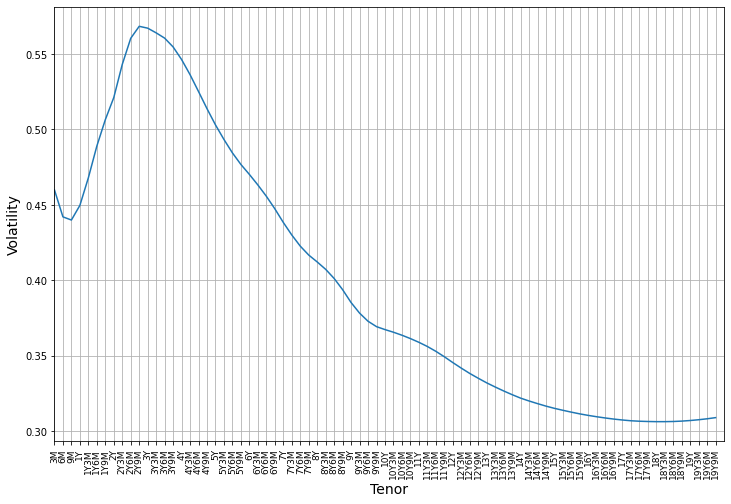
\includegraphics[width=1.1\linewidth]{cap_vola}
	\end{columns}
	\end{itemize}
\end{frame}

\begin{frame}{Swaptions}
	\begin{itemize}
		\item There are two main types of \textcolor{red}{swaptions} (as the underlying swaps), a \emph{payer} and a \emph{receiver} version.
		\item An \textcolor{red}{European payer swaption} is an option giving the right but not the obligation to enter a payer IRS at a given future time, called the \emph{swaption maturity}. If you are on the buyer side (you are long payer swaption) which is your view on rates ? Why ? And the receiver ?
		\item Usually, the swaption maturity coincides with the first reset date of the underlying IRS.
		\item The length of the underlying IRS is called the \emph{tenor} of the swaption.
	\end{itemize}
\end{frame}

\begin{frame}{An Example}
	\begin{itemize}
	\item A has raised a $10y$ loan with floating interest rate fixed every three months (IBOR + margin).
	\item A wants to \emph{hedge the loan against rising interest rates but also to benefit from the floating rate}, i.e. should fixed interest rates not rise above a certain level (the swaptions strike-rate $K$).
	\item The purchase of a payer swaption could hedge this risk: 
	\begin{columns}
	\column{0.45\linewidth}
	\begin{itemize}
		\item \textbf{interest rates increase}: A may exercise the swaption and be a party to an interest rate swap as a payer of a fixed rate of interest;
	\item \textbf{swap-rate below $K$}: it will not be exercised and A will continue to have floating-rate funding.
	\end{itemize}
	\column{0.45\linewidth}
	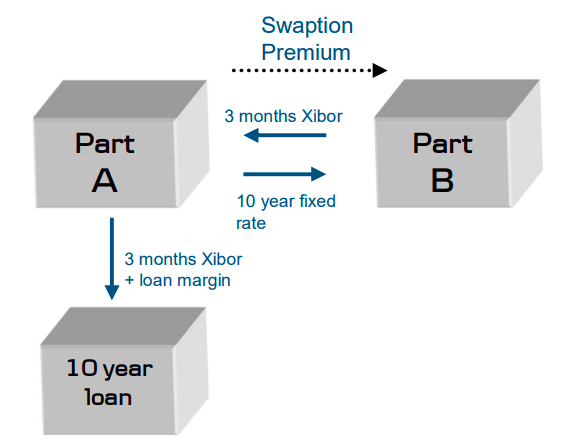
\includegraphics[width=1.\linewidth]{swaption_example}
	\end{columns}
\end{itemize}
\end{frame}

\begin{frame}{Swaptions Payoff}
	\begin{itemize}	
		\item We characterize the payoff in three different ways
		\begin{itemize}
			\item The swaption is said to be at-the-money (ATM) if
			\begin{equation*}
				K = K_{ATM} = S_{\alpha,\beta}(0) = \frac{P(0,T_\alpha)-P(0,T_\beta)}{\sum_{i=\alpha+1}^\beta \tau_i P(0,T_i)}
			\end{equation*}
			where $T_\alpha$ is the maturity of the swaption, and $T_\beta$ the last payment date of the underlying swap (the first being $T_{\alpha+1})$. That is when the strike is equal to the swap forward rate $S_{\alpha,\beta}(t)$.
			\item The payer swaption is in-the-money if $K<K_{ATM}$ and out-of-the-money otherwise.
			\item The opposite holds for the receiver swaption.
		\end{itemize}
		\item ATM swaption are quoted for maturities ranging between $1m$ and $30y$, and for tenors between $1y$ and $30y$.
	\end{itemize}
\end{frame}

\begin{frame}{Swaption as an Option on a Swap}
	\begin{itemize}
		\item The discounted payoff of a payer swaption (with maturity $T_\alpha$) is given, recalling the value of a payer IRS ($
			\sum_{i=\alpha+1}^\beta P(T_\alpha,T_i)\tau_i (F(T_\alpha,T_{i-1},T_i) - K)$)
		by
		\begin{equation}
			D(t,T_\alpha)\left(\sum_{i=\alpha+1}^\beta P(T_\alpha,T_i)\tau_i (F(T_\alpha,T_{i-1},T_i) - K)\right)^+
		\end{equation}
		\item This payoff cannot be easily decomposed in elementary parts but it can be rewritten in a different way
%		\begin{equation}
%			ND(t,T_\alpha)\left(S_{\alpha,\beta}(T_\alpha)-K\right)^+\sum_{i=\alpha+1}^\beta \tau_i P(t,T_i)
%		\end{equation}
	\end{itemize}
\end{frame}

\begin{frame}{Swaption as an Option on a Swap}
	\begin{itemize}
			\item Recall that we have expressed the swap payoff also as $
					\sum_{i=\alpha+1}^\beta \tau_i P(t,T_i)(S_{\alpha,\beta}-K)$
					
			\item If we look at the swaption payoff in this way and we model directly $S_{\alpha,\beta}(t)$ instead of $F(t, T_{i-1},T_i)$ we can write the swaption price as the expectation of the following
			\begin{equation}
					\left[D(t,T_\alpha)\sum_{i=\alpha+1}^\beta \tau_i P(t,T_i)\max(S_{\alpha,\beta}(T_\alpha)-K, 0)\right]
				\end{equation}
			which seems easier and more intuitive.
		\end{itemize}
\end{frame}

%\begin{frame}{Swaption as an Option on a Swap}
%	\begin{itemize}
%		\item So the forward rates are the chosen state variable, also the correlation between them is needed...
%		\item Market practice: approximation formula (see chapter 6 of Brigo-Mercurio) the definitive reference for this issue.
%		\item Clearly here a model which accounts for terminal correlations needed.
%		\item Which is the relationship between a Cap and a payer swaption with the same payment and roll dates ?
%	\end{itemize}
%
%\end{frame}


\begin{frame}{Differences between Caps and Swaptions}
	\begin{itemize}
		\item As we have seen caps can be decomposed into more elementary products: \textcolor{red}{caplets}. You can value simply each caplet at once and then add their prices
		\begin{itemize}
			\item you can value them modeling each forward rate at once;
			\item \textbf{no joint action of forward LIBOR rates is involved.}
		\end{itemize}
		\item Unfortunately this is not possible in swaptions.
		\item Swap rates are almost a weighted average of forward rate and hence observes that the volatility of the swap rate should depend on the forward rate volatilities as well as their correlation.
		%\item if you take as fundamental entity the LIBOR rates you ahve to deal with the joint action of the simple forward LIBOR rates. 
		\item So you have to \textbf{deal with terminal correlation} between rates of different portions of the yield curve. %Can you provide an example ?
	\end{itemize}
\end{frame}

\begin{frame}{Swaption as an Option to Exchange Fixed with Floater}
	\begin{itemize}
		\item We have seen that a Swap can be viewed as an exchange of bonds (fixed for floater).
		\item Hence a Swaption is an option to exchange fixed for floating bonds (or viceversa).
		\item We need an expression for a \textcolor{red}{Coupon Bond Option}.
		\item But if we could express a Coupon Bond Option as a Portfolio of Zero Coupon Bond Options life would be simpler as most models have losed formula for the latter but not the former.
		\item We can do that thanks to a recipe known as \textcolor{red}{Jamshidian's decomposition}.
	\end{itemize}
\end{frame}

\begin{frame}{Jamshidian's Trick}
	\begin{block}{Jamshidian's Decomposition}
		Consider a sequence of functions $f_i$, a random variable $W$ and a constant $K\ge0$. If $f_i$ are monotone (decreasing), that is $\frac{\partial f_i}{\partial W} < 0;\;\forall i$, then 
		\begin{equation*}
			\left(K - \sum_i f_i(W)\right)^+ = 	\sum_i \left(K - f_i(W)\right)^+
		\end{equation*} 
		In financial terms it means that the payoff of an option on a portfolio of assets can be expressed in terms of a portfolio of options on each asset.
	\end{block}
\end{frame}

\begin{frame}{Jamshidian's Trick Proof}
	\begin{itemize}
	\item Since $\sum_i f_i$ is also monotone decreasing there is a unique solution $w$ to $\sum_i f_i(w) = K$.
	\item Finally since each $f_i$ is decreasing
	\begin{equation*}
		\begin{aligned}
		\left(K - \sum_i f_i(W)\right)^+ &= \left(\sum_i (f_i(w) -  f_i(W))\right)^+ = \\ 
		&= \sum_i (f_i(w) - f_i(W))\mathbb{1}_{W\le w} = \\ 
		&= \sum_i \left(K - f_i(W)\right)^+
		\end{aligned}
	\end{equation*}
\end{itemize}
\end{frame}

\begin{frame}{Back to Coupon Bond Option}
	\begin{itemize}
		\item Consider a coupon bond which pays the following cash flows $\mathcal{C}+[c_1,\dots,c_n]$ at dates $T=\{T_1,\ldots,T_n\}$].
		\item Let $t\leq T_1$, the bond price is given by
		\begin{equation*}
			CB(t,\mathcal{C},T)=\sum_{i=1}^n c_i P(t,T_i) =\sum_{i=1}^n c_i \Pi(t, T_i, r(T))
		\end{equation*}
		\item Suppose we would like to calculate the price of a put option with strike $K$ on this coupon bond. The payoff reads
		\begin{equation*}
			\left[K-CB(t,\mathcal{C},T)\right]^+
		\end{equation*}
	\end{itemize}
\end{frame}

\begin{frame}{Back to Coupon Bond Option}
	\begin{itemize}
		\item Now apply the Jamshidian's decomposition to the previous payoff
		\begin{equation*}
			\left[K-\sum_{i=1}^n c_i \Pi(t, T_i, r(T))\right]^+
		\end{equation*}
		\item So first let's find $r^*$ such that $\sum_{i=1}^n c_i \Pi(t, T_i, r^*) = K$
		\item If the model satisfies this condition
		\begin{equation*}
			\frac{\partial \Pi(t,T,r(t))}{\partial r}<0,\;\forall 0<t<s
		\end{equation*}
		we could rewrite the payoff as\ldots
		\end{itemize}
\end{frame}

\begin{frame}{Back to Coupon Bond Option}
	\begin{equation*}
		\sum_{i=1}^n c_i [\Pi(t, T_i, r^*)-\Pi(t, T_i, r(T))]^+
	\end{equation*}
	\begin{itemize}
		\item This equation tells us that we can price a coupon bond option as a portfolios of options on ZCBs.
		\item The strike of these option is calculated as the value of a ZCB given a \emph{particular} value of the short rate, and can be  calculated with a root finding procedure.
		\item In formulas the CBO with maturity $T$, strike $K$ reads
		\begin{equation}
			CBO(t,T,T_i,\mathcal{C},K) = \sum_{i=1}^n c_i ZBP(t,T,T_i,\Pi(T,T_i,r^*))
		\end{equation}
	\end{itemize}
\end{frame}

\begin{frame}{Adapting the Procedure to Swaptions}
	\begin{itemize}
		\item When interest rates are modeled using \textcolor{red}{Affine Short Rate Models} it is rather simple to arrive to the swaption price formula.
		\item \emph{Affine Models} indeed relates ZCB price to a spot rate model according to 
		\begin{equation*}
			P(t,T) = A(t,T)e^{-B(t,T)r}
		\end{equation*} 
		\item Hence the value $r^*$ can be determined as a solution of 
		\begin{equation*}
		\sum_{i=1}^n A(t,t_i)e^{-B(t,t_i)r^*}
		\end{equation*}		
%%		\item Denote as usual with $\tau_i$ the year fraction between $t_{i-1}$ and $t_i$, fix $c_i=X\tau_i$ and $c_n = 1+X\tau_i$.
%%		\item Let the swap notional be equal to N.
%%		\item Thus for the price of a payer swaption we have to calculate the following payoff
%%		\begin{equation*}
%%			\left[1-CB(t,\mathcal{C},T)\right]^+
%%		\end{equation*}
%%		\item We can calculate this payoff via the procedure outlined before.
	\end{itemize}
\end{frame}

\begin{frame}{Swaption Pricing via Affine Short Rate Models}
	\begin{itemize}
		\item Given the affine structure of the model, we get
		\begin{equation*}
			K_i = A(t,t_i)e^{-B(t,t_i)r^*}
		\end{equation*}
		\item The payer swaption price is thus given by
		\begin{equation}
			PS(t,T,N) = N\sum_{i=1}^n ZBP(t,T,t_i,K_i)
		\end{equation}
		while the receiver swaption price reads
		\begin{equation}
			RS(t,T,N) = N\sum_{i=1}^n ZBC(t,T,t_i,K_i)
		\end{equation}
	\end{itemize}
\end{frame}

\begin{frame}{Black Formula for Swaptions}
	\begin{itemize}
		\item Replacing the forward rate $F(0, t_{i-1}, t_i)$ with the swap rate $S_{\alpha,\beta}(0)$ and plugging in the quoted swaption volatility you get Black's formula for swaptions
		\begin{equation}
			\begin{aligned}
			PS_{Bl}(0,T,&S,N,K,\sigma_{\alpha,\beta})=\\
			&N\sum_{i=\alpha+1}^\beta P(0,T_i)\tau\left[S_{\alpha,\beta}(T)\Phi(d_1)-K\Phi(d_2)\right]
		\end{aligned}	
		\end{equation}
		where
		\begin{equation*}
			d_{1,2} = \frac{\log{\frac{S_{\alpha,\beta}}{K}} \pm \frac{v^2}{2}}{2}
		\end{equation*}
		and
		\begin{equation*}
			v = \sigma_{\alpha,\beta}\sqrt{T_\alpha}
		\end{equation*}
	\end{itemize}
	In the market $\sigma_{\alpha,\beta}$ is quoted: here however we have one more dimension with respect to caps.
\end{frame}

\begin{frame}{Swaptions Volatility Calibration}
	\begin{itemize}
		\item Swaption volatilities are quoted for different maturities and tenors (length of th underlying swaps).
		\item Both for ATM and away from ATM in both sides (swaption smile).
		\item So swaption have an additional dimension with respect to caps.
		\item They have also a different \emph{delta} effect on your book.
		%		\item Volatility trade between caps ans swaption: WEDGE
	\end{itemize}
	\begin{tikzpicture}[remember picture,overlay]
		\node[xshift=5cm,yshift=-3.7cm] (image) at (current page.center) {
\includegraphics[width=20px]{python_logo}};
		\node[align = center, yshift=1.45cm, below=of image] {\tiny{\href{shorturl.at/iFMW9}{shorturl.at/iFMW9}}};
	\end{tikzpicture}	
\end{frame}

\begin{frame}{Bermudan Swaptions}
	\begin{itemize}
		\item It is a swaption in which the optionality can be exercised at a predetermined set of dates (not only one).
		\item It is useful for hedging callable bonds (especially if step-up, i.e. with the coupon increasing with time).
		\item A \textcolor{red}{Bermudan Swaption} gives the holder the right but non the obligation to enter in an interest rate swap contract at different dates (usually the swap reset dates) with some days of notification to the counter-party.
		\item The interest rate swap the holder can enter into, is the same existing contract, so if the holder does not exercise at the first date in the call schedule, the option for the following periods is written on shorter swaps.
	\end{itemize}
\end{frame}

\begin{frame}{Bermudan Swaption Example}
	\begin{itemize}
		\item As an example consider the following: receiver Bermudan Swaption written on a 3 years swap with the first call date $2y$ from now (we suppose semi-annual payments).
		\item If at the end of the second year she will not exercise, six months later she will have to decide if enter or not in the same remaining swap which now has become a $2y6m$ swap.
		\item In this case at the last option exercise date she will decide whether or not to enter on the $2y6m-3y$~$FRA$.
	\end{itemize}
\end{frame}		

\begin{frame}{Bermudan Swaption Payoff}
	\begin{itemize}
		\item At the maturity $T$, the payoff of a Bermudan swaption is given by
		\begin{equation*}
			BS(T) = \max(0, V_{\text{swap}(T)})
		\end{equation*}
		where $V_{swap}(T)$ is the value of the underlying swap at $T$.
		\item At any exercise date $T_i$, the payoff of the Bermudan swaption is given by
		\begin{equation*}
			BS(T_i) = \max(K(T_i), V_{\text{swap}(T_i)})
		\end{equation*}
		where $V_{\text{swap}(T_i)}$ is the exercise value of the Bermudan swap and $K(T_i)$ is the intrinsic value, i.e. the holder of the option receives $\max(K(T_i), 0)$ if the option is exercised at time $T_i$.
	\end{itemize}
\end{frame}

\begin{frame}{Bermudan Swaption Pricing}
	\begin{itemize}
		\item Some interest rate instruments can be priced just looking at the term structure (FRA and SWAPS).
		\begin{itemize}
			\item The only problem is: which is the right term structure ? (this is a lesson from the 2008 crisis) 
		\end{itemize}
		\item Some other instruments cannot be priced only with the yield curve: we need the future (risk-neutral) evolution of the rates.
		%\item Non-linearities come in !
		%\item Swaptions are non-linear products and may require to model the correlation between forward LIBOR rates.
		\item Given the complexity of Bermudan swaption valuation, there is no closed form solution. Therefore, we need to select an interest rate term structure model and a numeric solution to price this contract numerically.		
		\item Typically tree techniques or the Longstaff-Schwartz method are used.
	\end{itemize}
%The issuer has an option which it pays for by offering a higher coupon rate. If interest rates in the market have gone down by the time of the call date, the issuer will be able to refinance its debt at a cheaper level and so will be incentivized to call the bonds it originally issued.[2] Another way to look at this interplay is that, as interest rates go down, the present values of the bonds go up; therefore, it is advantageous to buy the bonds back at par value.
\end{frame}

\begin{frame}{Callable Coupon Bond}
	\begin{itemize}
		\item A \textcolor{red}{callable bond} is a bond in which, on the call date(s) (there can be more than one), the issuer has the right, but not the obligation, to buy back (redeem) the bonds from the bond holders at a defined call price.
		\item We have seen that a swap can be regarded as an exchange of bonds. It is easy to guess that a replica for the callable bond price can be obtained by simply adding a Swaption to the swap used to price a bond.
		\item If there are multiple callability dates is clear that the swaption we need is a bermudan one.
		\item With a receiver bermudan swaption with the same contractual conventions of the Swap (so the strike of the swaption is equal to the coupon of the bond) we can offset the swap; which represents the economic equivalent of calling the bond at par.
		%\item So $\max(CCBP(T,S,K,\tau)-100, 0)$ can be represented as $\max(K-S(T_j,\beta)(T), 0)$.
		%\item Intuition: long on the bond, short on the rates.
	\end{itemize}
\end{frame}

\begin{frame}{Callable vs Non Callable Coupon Bonds}
	\begin{itemize}
		\item \emph{Ceteris paribus} a non callable coupon bond has an higher price than a callable one because the callability option adds value to an issuer
		\begin{equation*}
		\text{price of callable bond} = \text{price of straight bond} – \text{price of call option}.
		\end{equation*}
		\item At inception both must be worth 100 (a part from other costs and fees which we will neglect).
		\item A typical coupon bond, once credit risk is isolated and remunerated, will pay the average market rates prevailing at the time of the issue. These are related to the swap rate prevailing at that moment (remember that the swap rate is sort of average of forward rates).
	\end{itemize}
\end{frame}

\begin{frame}{Callable vs Non Callable Coupon Bonds}
	\begin{itemize}
		\item Suppose credit risk is zero: in this ideal case the coupon bond will pay the corresponding swap rate prevailing on the market.
		If we price a $5y$ bond, at inception, the following must hold
		\begin{equation*}
			CBP(0,5,K,\tau)=100-NPV_{\text5y-swap(0)}=100
		\end{equation*}
		\item Which implies $NPV_{\text{5y-swap(0)}}=0$, hence $K=S_{\text{5y-swap(0)}}$. This means that credit consideration apart, a bank must pay the market prevailing rate when it issues a bond. And this should not surprise anyone.
	\end{itemize}
\end{frame}

\begin{frame}{Callable vs Non Callable Coupon Bonds}
	\begin{itemize}
		\item If the same bond were callable after two years each six months, we will have the following facts
		\item Let us denote $RBS(t,6m,T_{1c},T_\beta,K,N)$ the bermudan receiver swaption with first call date $T_{1c}$ and subsequent ones each six months. The last payment date is equal to the one of the swap.
		\item In this case the call dates vector is $[2y,2y6m,3y,3y6m,4y,4y6m]$.
		\item Suppose $RBS(0,6m,T_{2y},T_{5y},K_1,N)>0$
		\begin{equation}
			CBP(0,5,K,\tau)=100-(NPV_{\text{5y-swap(0)}}+NPV_{RBS})=100
		\end{equation}
		\item It implies 
		\begin{equation}
			\begin{gathered}
				NPV_{\text{5y-swap(0)}}=-NPV_{RBS}<0 \\
				K_1 > K_{\text{5y-swap(0)}}
			\end{gathered}
		\end{equation}
	\end{itemize}
\end{frame}

\begin{frame}{Risk Analysis of Callable Bonds}
	\begin{itemize}
		\item Coupons are better than market prevailing rates would have allowed for a fixed rate note.
		\item On the other hand, if interest rates fall, the bonds will likely be called and they can only invest at the lower rate, i.e. this is like writing (selling) an option, the option writer gets a premium up front, but has a downside if the option is exercised.
		\item After the bond issue if rates go down the bank will call the bond (because, ceteris paribus, it will have a price above 100) as it will not want to pay an higher than market level remuneration for the money it has borrowed from customers.
		\item Conversely if rates go down it will not buy back the bond as in financing itself at a lower than market implied rates.
		%The call price will usually exceed the par or issue price. In certain cases, mainly in the high-yield debt market, there can be a substantial call premium.
		
		
		%The largest market for callable bonds is that of issues from government sponsored entities. They own many mortgages and mortgage-backed securities. In the U.S., mortgages are usually fixed rate, and can be prepaid early without cost, in contrast to the norms in other countries. If rates go down, many home owners will refinance at a lower rate. As a consequence, the agencies lose assets. By issuing numerous callable bonds, they have a natural hedge, as they can then call their own issues and refinance at a lower rate.
		%\item It cannot go much above par. The price-yield relation is broken at a certain level.
		%\item Investors sells an option to the bank for higher (initial) coupons.
		\item Customer is long bond, short rates, short option (receiver swaption).
	\end{itemize}
\end{frame}

\begin{frame}{Few Useful Math Tricks}
	\renewcommand{\arraystretch}{1.4}
	\begin{table}[bt]
		\begin{tabular}{|c|c|} \hline
			rule 1 & $\max(F(T),K) = K + \max(F(T) -K, 0)$\\ \hline		
			rule 2 & $\max(F(T)-K,0) = F(T)-K + \max(K-F(T), 0)$\\ \hline		
			rule 3 & $\max(\alpha F(T),K) = \alpha \max(F(T),\frac{K}{\alpha})$\\ \hline		
			rule 4 & $\max(\alpha F(T),K) = K + \alpha\max(F(T)-\frac{K}{\alpha}, 0)$\\ \hline		
			rule 5 & $\min(\max(F(T),0)) = -\min(-F(T),0)$\\ \hline		
			rule 6 & $\begin{aligned}&\min(\max(F(T)-K_{\max}, 0), K_{\min}) =\\ &\max[F(T)-K_{\max},0]-\max[F(T)-K_{\max}-K_{\min},0]\end{aligned}$\\ \hline		
		\end{tabular}
	\end{table}
\end{frame}

%A position in options (a situation/ relationship expressed originally as vega) in which any increase in the implied volatility of the underlying asset will generate a profit, even without a move in the underlying asset.

\begin{frame}{Reverse Floater Bond}
	\begin{itemize}
		\item Denote with $F(T)$ the EURIBOR 6m observed in $T$. We can write the \textcolor{red}{Reverse Floater} coupon in general form as
		\begin{equation}
			\mathcal{C}=\max[0, K-\alpha F(T)]
		\end{equation}
		\item Which, adding and subtracting $K$, can be rewritten as
		\begin{equation*}
			\max[-K,-\alpha F(T)] + K = K - \min[K,\alpha F(T)]
		\end{equation*}
		\item Finally, after having added and subtracted $\alpha F(T)$
		\begin{equation*}
			\begin{aligned}
				K-&\min[0,K-\alpha F(T)]+\alpha F(T) \\ &= K - \alpha F(T) + \max[\alpha F(T)-K,0]
			\end{aligned}
		\end{equation*}
	\end{itemize}
\end{frame}

\begin{frame}{Reverse Floater Bond}
	\begin{itemize}
		\item Previous formula gives the payoff as the sum of a fixed leg of an IRS and Cap with strike $K$
		\begin{equation}
			\begin{aligned}
				K-&\min[0,K-\alpha F(T)]+\alpha F(T) \\ &= \underbrace{K - \alpha F(T)}_{\text{IRS fixed leg}} + \underbrace{\max[\alpha F(T)-K,0]}_{\text{Cap}}
			\end{aligned}
		\end{equation}
	\item Invest in an inverse floater when the reference rate is high and you expect it to decrease faster than the forwards imply or when the reference rate is low, the forwards are implying a steep increase but you don’t believe in it.
	\item Other typical investors are long vega, if $K$ is close to the forward rates, vega is much higher.
	%\item What happens if $F(T)$ collapses ? How the vega affects the bond holder ?
	\begin{tikzpicture}[remember picture,overlay]
	\node[xshift=5cm,yshift=-3.7cm] (image) at (current page.center) {
\includegraphics[width=20px]{python_logo}};
	\node[align = center, yshift=1.45cm, below=of image] {\tiny{\href{shorturl.at/wK368}{shorturl.at/wK368}}};
	\end{tikzpicture}	
	\end{itemize}
\end{frame}

\end{document}
